%! Author = mkeim
%! Date = 7/11/24

\section{Related Work} \label{sec:relatedwork}
\para{Tracking how word meanings change over time.}
The evolution of word meanings over time has been a subject of significant interest.
Researchers employed a diverse array of methodologies, including \emph{word embeddings} ~\cite{kulkarni2014statisticallysignificantdetectionlinguistic},
\emph{neural language models} ~\cite{kim-etal-2014-temporal}, and \emph{diachronic analysis} ~\cite{hamilton-etal-2016-diachronic, kutuzov-etal-2018-diachronic},
to track and examine semantic shifts across historical periods.
Much of this research utilized the \emph{Google Books Ngram corpus}
~\cite{gulordava-baroni-2011-distributional, kim-etal-2014-temporal, kulkarni2014statisticallysignificantdetectionlinguistic, 10.1007/978-3-319-50496-4_18, hamilton-etal-2016-cultural, hamilton-etal-2016-diachronic, kutuzov-etal-2018-diachronic},
a vast collection spanning from 1900 to 2009,
encompassing over 500 billion books in seven languages.
This dataset provides n-grams with corresponding yearly occurrences and frequencies.

\begin{figure}[tbh]
\vspace{-1em}
\centering
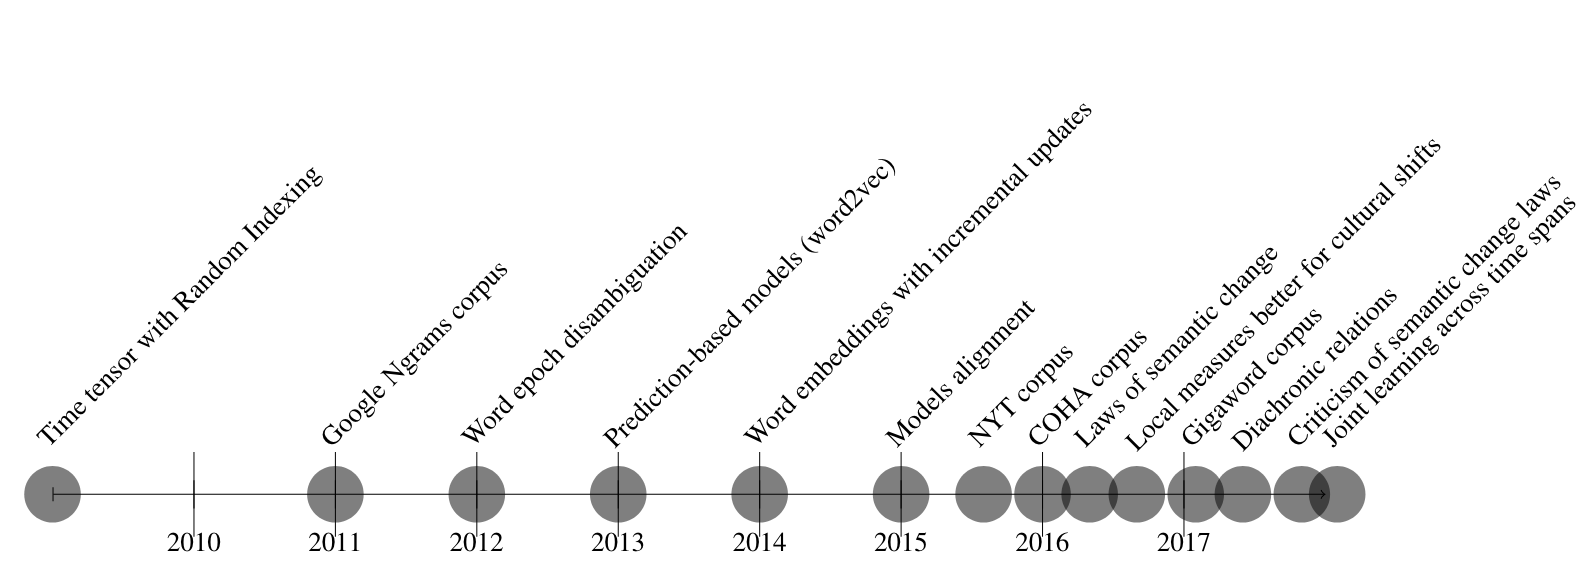
\includegraphics[scale=0.45]{figures/survey}
\caption{Timeline of models used to study semantic shifts (taken from \cite{kutuzov-etal-2018-diachronic})}\label{fig:testsvg}
\end{figure}

\para{Words can change meaning over time through several linguistic processes.}
Words have the ability to undergo shifts in meaning over the course of time as a result of various linguistic mechanisms,
including but not limited to:
\begin{itemize}
    \item \emph{semantic drift} ~\cite{gulordava-baroni-2011-distributional, kim-etal-2014-temporal, kulkarni2014statisticallysignificantdetectionlinguistic}
    \begin{itemize}
        \item Refers to the evolution of word \underline{\emph{meanings}} over time.
        \item Example: The word `gay' originally meant `happy' or `carefree', but now it predominantly means `homosexual'.
    \end{itemize}
    \item \emph{syntactic alterations} ~\cite{kulkarni2014statisticallysignificantdetectionlinguistic, hamilton-etal-2016-cultural, giulianelli-etal-2020-analysing}
    \begin{packed_itemize}
        \item Syntax focuses on the \underline{\emph{structure}} of language.
        This type of change pertains to modifications in the arrangement of words in sentences.
        \item Example:  The word `apple', which transitioned from being used as a `common noun' (e.g., a fruit) to a `proper noun' (referring to the Apple company) after the company’s rise in the 1980s.
    \end{packed_itemize}
    \item \emph{broadening} ~\cite{kulkarni2014statisticallysignificantdetectionlinguistic, hamilton-etal-2016-cultural, giulianelli-etal-2020-analysing}
        \begin{itemize}
            \item A word’s meaning becomes more general than its earlier meaning, also known as \underline{\emph{generalization.}}
            \item Example: `Holiday' originally meant a religious festival, but now it can refer to any day of celebration or time off.
        \end{itemize}
    \item \emph{narrowing} ~\cite{kulkarni2014statisticallysignificantdetectionlinguistic, giulianelli-etal-2020-analysing}
    \begin{itemize}
            \item A word’s meaning becomes more specific than its earlier meaning, also known as \underline{\emph{specialization}}.
            \item Example: `Literally' used to mean `figuratively' or `symbolically'.
            Now, it is used to emphasize the truthfulness of a statement.
        \end{itemize}
    \item \emph{amelioration}
     \begin{itemize}
            \item A word takes on a more \underline{\emph{positive}} meaning over time.
            \item Example: The word `thrifty' once meant `cheap' but now suggests responsible use of resources.
        \end{itemize}
    \item \emph{pejoration} ~\cite{10.1162/opmi_a_00081, gulordava-baroni-2011-distributional}
        \begin{itemize}
            \item A word takes on a more \underline{\emph{negative}} meaning over time.
            \item Example: The word `awful' meant `full of awe' which transitioned to `terrible' or `appalling'.
        \end{itemize}

\end{itemize}

Hamilton et al.\ (2016) highlighted that \emph{cultural} or \emph{linguistic} factors could have driven these transformations.
Certain studies concentrated on semantic changes, some worked on syntactic changes, ~\cite{kulkarni2014statisticallysignificantdetectionlinguistic, hamilton-etal-2016-cultural, 10.1162/opmi_a_00081}
and others explored the broader evolution that words underwent ~\cite{gulordava-baroni-2011-distributional, kim-etal-2014-temporal, kulkarni2014statisticallysignificantdetectionlinguistic, hamilton-etal-2016-diachronic}.
\Cref{tab:related-work} outlines various types of linguistic changes and the approaches employed to identify them.

% ------------------------------------------------------------------ SEMANTIC ------------------------------------------------------------------
\subsection{Semantic Drift} \label{subsec:semantic-drift}
\para{Building on the extensive research on \emph{semantic} change.}
Semantic change refers to any change in the meaning(s) of a word over time or acquiring a new sense ~\cite{gulordava-baroni-2011-distributional, 10.1162/opmi_a_00081}.
Kutuzov et al.\ (2018) conducted a survey on semantic shifts, consolidating the existing academic research in this domain.
Their work provides a comprehensive overview of the methodologies and findings related to tracking semantic changes over time using computational techniques.

\begin{table}[]
\centering
\small
\begin{tabular}{@{}llllll@{}}
\toprule
\multicolumn{1}{c}{\textbf{Linguistic}}              & \multicolumn{1}{c}{\textbf{Approach}}                                            & \multicolumn{1}{c}{\textbf{TCD}}      & \multicolumn{3}{c}{\textbf{Example}}                                                                                                                                                                              \\ \cmidrule(l){4-6}
\multicolumn{1}{c}{\textbf{Change}}                  & \multicolumn{1}{c}{\textbf{}}                                                    & \multicolumn{1}{c}{\textbf{}}         & \textbf{Word}             & \textbf{Former Usage}                                                                         & \textbf{New Usage}                                                                    \\ \midrule
\rowcolor{lightgray}                                 & \multicolumn{5}{c}{\textbf{FREQUENCY \cite{gulordava-baroni-2011-distributional, kulkarni2014statisticallysignificantdetectionlinguistic, hamilton-etal-2016-diachronic}}}                                                                                                                                                                   \\
\textbf{\textbf{Semantic}}                           & Log Ratio                                                                        & 1960 \& 1990                          & disk                      & -                                                                                             & -                                                                                     \\ \cmidrule(l){2-6}
\textbf{}                                            & Word Frequency                                                                   & 1900--2005                            & bitch                     & female dog                                                                                    & slang                                                                                 \\ \cmidrule(l){2-6}
\rowcolor{lightgray}                                 & \multicolumn{5}{c}{\textbf{DISTRIBUTIONAL \cite{gulordava-baroni-2011-distributional, kim-etal-2014-temporal, kulkarni2014statisticallysignificantdetectionlinguistic, 10.1007/978-3-319-50496-4_18, hamilton-etal-2016-diachronic, hamilton-etal-2016-cultural, 10.1162/opmi_a_00081, giulianelli-etal-2020-analysing}}}                                                                                                                    \\ \cmidrule(l){2-6}
\textbf{}                                            & \begin{tabular}[c]{@{}l@{}}Local Mutual \\ Information\end{tabular}              & 1960 \& 1990                          & sleep                     & deep sleep                                                                                    & sleep disorder                                                                        \\ \cmidrule(l){2-6}
\textbf{}                                            & \begin{tabular}[c]{@{}l@{}}Continuous Word \\ Embeddings\end{tabular}            & 1900--2009                            & cell                      & closet, dungeon                                                                               & phone, cordless                                                                       \\ \cmidrule(l){2-6}
\textbf{}                                            & \begin{tabular}[c]{@{}l@{}}Change Point \\ Algorithm\end{tabular}                & 1900--2005                            & gay                       & cheerful, dapper                                                                              & \begin{tabular}[c]{@{}l@{}}lesbian, \\ homosexual\end{tabular}                        \\ \cmidrule(l){2-6}
\textbf{}                                            & Clustering (DBSCAN)                                                              & 1900--2000                            & mouse                     & mice, rat                                                                                     & cursor, pointer                                                                       \\ \cmidrule(l){2-6}
\textbf{}                                            & \begin{tabular}[c]{@{}l@{}}Cultural and \\ Linguistic Drift\end{tabular}         & 1800--2000                            & virus                     & \begin{tabular}[c]{@{}l@{}}infected with virus\end{tabular}                                   & \begin{tabular}[c]{@{}l@{}}spreading\\  computer virus\end{tabular}                   \\ \cmidrule(l){2-6}
\textbf{}                                            & \begin{tabular}[c]{@{}l@{}}Diachronic Word\\ Embeddings\end{tabular}             & 1800--1999                            & awful                     & full of awe                                                                                   & terrible or appalling                                                                 \\ \cmidrule(l){2-6}
\textbf{}                                            & \begin{tabular}[c]{@{}l@{}}Contextual Word \\ Embeddings\end{tabular}            & 1910 – 2009                           & tenure                    & \begin{tabular}[c]{@{}l@{}}short term leases,\\ insecurity of tenure\end{tabular}             & \begin{tabular}[c]{@{}l@{}}tenure of office, \\ employment \end{tabular}              \\ \cmidrule(l){2-6}
\textbf{}                                            & \begin{tabular}[c]{@{}l@{}}Semantic Similarity \\ Analysis\end{tabular}          & 2014--2022                            & immunity                  & \begin{tabular}[c]{@{}l@{}}politics (‘legislator’,\\ ‘representative’).\end{tabular}          & \begin{tabular}[c]{@{}l@{}}health-related \\ (‘prevention’, ‘AIDS’)\end{tabular}      \\ \cmidrule(l){2-6}
\rowcolor{lightgray}                                 & \multicolumn{5}{c}{\textbf{PART OF SPEECH \cite{kulkarni2014statisticallysignificantdetectionlinguistic, hamilton-etal-2016-cultural}}}                                                                                                                                                                                                      \\
\textbf{Syntactic}                                   & POS Tags                                                                         & 1900--2000                            & windows                   & \begin{tabular}[c]{@{}l@{}}doors and \\ windows of a house\end{tabular}                       & Microsoft Windows                                                                     \\ \midrule
\textbf{}                                            & \begin{tabular}[c]{@{}l@{}}Mixed-model \\ Regressions\end{tabular}               & 1800--2000                            & actually                  & originally, nominally                                                                         & presumed, believe\\
\bottomrule
\end{tabular}

\caption{\textbf{Comparative overview of linguistic change detection approaches.}
This table provides a comprehensive summary of various approaches and contributions to the study of linguistic changes,
categorizing the type of changes (semantic or syntactic), and the methodologies used, including frequency, distributional and part of speech approaches.
It highlights each study’s methods, such as word embeddings, statistical analysis, and clustering, along with the time periods of change detection (TCD) and examples of words.}
\label{tab:related-work}
\end{table}
\raggedbottom
%\vspace{-1em}

\para{Investigating semantic shifts through word contexts.}
Gulordava and Baroni (2011) detected semantic change by focusing on words used in the 1960s and 1990s.
They compared the similarity of the surrounding words (words that co-occur with the target word) in these two time periods.

To assess similarity, the researchers calculated the \emph{Local Mutual Information (LMI)} score between the central word and its surrounding words.
A low LMI score between the target word and its surrounding words across the two time periods indicated a potential semantic shift.
The study demonstrated that their distributional similarity models were effective in capturing \emph{cultural shifts} in word meaning.
For example, they found that the word `sleep' acquired more negative connotations related to sleep disorders when comparing its contexts in the 1960s to those in the 1990s.

\para{Tracking meaning evolution through neural nets.}
Kim et al.\ (2014) focused on analyzing how word meanings evolved between 1900 and 2009.
They developed the first method that employed \emph{prediction-based model} to trace semantic shifts.
This involved training a model on data from a specific year $y_i$ and then using the resulting word vectors as the starting point for training the model on the next year's data $y_i+1$.

Their method analyzed \emph{global shifts} in a word's vector semantics.
Additionally, by plotting the time series of a word's distance to its neighboring words in the model's vector space, they visualized the period during which the semantic shift occurred.
They demonstrated this for the word `cell' compared to its early neighbors, `closet' and `dungeon,' and the more recent neighbors, `phone' and `cordless.'
For `cell,' the identified period of change (1985-2009), which interestingly coincides with the introduction and widespread adoption of cell phones by the public.

\para{Pinpointing significant shifts statistically.}
Kulkarni et al.\ (2015) proposes a novel computational approach to identify and quantify the semantic and usage changes in words across various media (new products, movies and books).
Building on the concept of distributed representations proposed by Hinton ~\cite{hinton1986learning}, they map words into a continuous vector space where words with similar meanings are positioned close together.
The approach hinges on constructing \emph{property time series} for each word.
They propose three methods for constructing these time series (\Cref{sec:paper_hamilton}):
\begin{packed_enumerate}
    \item \textbf{Frequency:}
    This method analyzes changes in a word's overall frequency of use, assuming a sudden shift in frequency might indicate a semantic shift.
    \item \textbf{Syntactic:}
    This method examines the distribution of a word's part-of-speech tags (e.g., noun, verb) across different time periods, aiming to capture changes in how the word functions grammatically.
    \item \textbf{Distributional:}
    This approach leverages word embeddings which are created for each year, and then alignment is done to represent them in joint embedding space,
    and it's utilized to construct distributional time series for a word's displacement.
\end{packed_enumerate}
Finally, they employed statistically sound \emph{change point detection algorithm} to identify significant moments in these time series, pinpointing the periods where word meaning or usage likely underwent a shift.
Their results indicated that computational methods for the detection of semantic shifts can be robustly applied to time spans less than a decade.

\para{Word semantic modelling of polysemant.}
Liao and Cheng (2016) explored the semantic changes of words.
Their approach built on the understanding that word meaning is closely tied to its context.
When a word's meaning changes, the surrounding words used with it \emph{(context words)} are likely to change as well.
They focused on \emph{polysemous} words (words with multiple meanings) and aimed to detect when new meanings emerged.

They used the \emph{skip-gram architecture with negative sampling} ~\cite{10.5555/2999792.2999959} to obtain word embeddings.
This technique helped in capturing the contextual meaning of words by representing them in a continuous vector space.
They employed \emph{DBSCAN} to group word embeddings.
DBSCAN helped in identifying clusters of similar word contexts and distinguishing them from noise, which could indicate semantic changes.
To find similar words, they used a nearest neighbor search method called \emph{Random Project Forest}.
This method helped in identifying words that are contextually similar to a given word.
 Finally, they compared the stability of \emph{similar words} with the stability of their \emph{context words}.

\para{Distinguishing cultural shifts from linguistic drift.}
Hamilton et al.\ (2016) addressed the challenge of distinguishing between \emph{cultural shifts} and \emph{linguistic drift}, both of which can contribute to semantic change.
They proposed two distinct measures based on distributional representations to distinguish between these two types of semantic change:
\begin{packed_enumerate}
    \item \textbf{Local neighborhood masure:}
    This measure focused on the closest neighbors (most similar words) in a word's embedding.
    A drastic shift in these nearest neighbors suggests a significant change in core meaning, potentially driven by a \emph{cultural shift}
    (e.g., `gay' changing from carefree to referring to homosexuality).
    \item \textbf{Global measure:}
    This measure considered the overall distribution of a word's surrounding words in a larger context window.
    Gradual changes in this broader distribution are more likely to reflect \emph{linguistic drift}, the natural evolution of language due to regular processes
    (e.g., `promise' expanding from a declaration to also suggesting a likelihood).
\end{packed_enumerate}
Prior research often treated semantic change as a single phenomenon.
Hamilton et al.\ offered a novel approach by distinguishing between cultural shifts and linguistic drift using their two measures.

\para{Diachronic analysis on historical data: }
The primary goal of Hamilton et al.\ (2016) is to track semantic changes and understand how the meanings of words shift in different historical contexts.
They created word embeddings for different time periods using both the PPMI matrix with SVD and the SGNS model.
These embeddings were generated from historical text corpora to capture the contextual usage of words in each period.
After creating the embeddings, they aligned the embeddings.
Once the embeddings are aligned, they calculate the \emph{semantic displacement} of a word.
This essentially measured how much a word's vector representation has moved in the embedding space between two time periods.
The study demonstrates that their method effectively identified semantic change in words and uncovered two statistical `laws' of semantic change:
\begin{packed_enumerate}
    \item \textbf{Law of Conformity}, which suggests that the rate of semantic change is inversely proportional to a word's frequency.
    High-frequency words tend to change meaning more slowly.
    \item \textbf{Law of Innovation}, on the other hand, proposes that words with multiple meanings are more likely to undergo semantic transformations over time.
\end{packed_enumerate}
They leveraged the rich information within word embeddings to quantify the degree of semantic change (semantic displacement) and identified potential patterns.

\para{Semantic shifts with contextual embeddings:}
Giulianelli et al.\ (2020) explored the phenomenon of lexical semantic change using an unsupervised approach using \emph{BERT}.
They utilized the \emph{BERT} model to generate contextual word embeddings, which captured the meaning of a word based on its surrounding context.
The extracted word usage vectors are then clustered into different \emph{usage types} using the \emph{k-means clustering algorithm}.
This helped to identify distinct senses or meanings of the words as they appear in various contexts.
They analyzed these clusters for a specific word across different time periods.
The study proposed three metrics to quantify semantic change:
\begin{packed_enumerate}
    \item \textbf{Entropy Difference (ED)}: Measures the change in uncertainty (entropy) of a word’s usage distribution over time.
    \item \textbf{Jensen-Shannon Divergence (JSD)}: Compares the similarity of word usage distributions across time intervals.
    \item \textbf{Average Pairwise Distance (APD)}: Computes the average distance between word usage vectors from different periods, indicating shifts in word meaning.
\end{packed_enumerate}
The qualitative analysis indicated that the approach could capture various linguistic phenomena, including both synchronic (current usage) and diachronic (historical changes) aspects.

\para{Semantic similarity:}
The impact of significant events like the COVID-19 pandemic on language and semantic change has also been a subject of study.
Laurino et al.\ (2023) explores tracking fast semantic changes through a large-scale word association task, aiming to understand how the collective mental lexicon evolves in response to such global events.
Their research highlights the dynamic nature of language and how it incorporates new senses.
One key finding from their work is that words directly related to the pandemic exhibited a greater difference in semantic similarity between pre-pandemic and pandemic time periods.
This suggests that these words underwent a more significant and rapid semantic shift compared to control words not associated with the pandemic.
They also employ semantic similarity analysis to quantify the shifts in meaning for pandemic-related words and provides evidence that the COVID-19 pandemic acted as a catalyst for rapid semantic change.
For instance, words like `quarantine', `mask', and `social distancing' took on new and prominent meanings in everyday conversation.

\subsection{Takeaways}\label{subsec:semantic-takeaways}
Existing research on semantic change detection employs a diverse range of methods.
Traditional approaches rely on frequency analysis, such as log ratio computations\cite{gulordava-baroni-2011-distributional},
while more recent studies utilized distributional representations\cite{kim-etal-2014-temporal, kulkarni2014statisticallysignificantdetectionlinguistic, hamilton-etal-2016-cultural},
including word embeddings generated by techniques like SGNS, PPMI, and SVD\cite{hamilton-etal-2016-diachronic}.
Clustering algorithms like DBSCAN\cite{10.1007/978-3-319-50496-4_18} was applied to detect semantic shifts in polysemous words.
By clustering words based on their contextual similarity, they were able to identify when a word’s meaning had shifted, as changes in clusters indicated emerging or evolving senses.
BERT-based contextual embeddings\cite{giulianelli-etal-2020-analysing} measured lexical semantic change by capturing how word meanings shift subtly across different contexts.
The advent of word embeddings provided a quantitative framework for measuring semantic change,
leading to the identification of patterns like the \emph{law of conformity} and \emph{law of innovation} as proposed by Hamilton et al.\ (2016).
These methods have successfully identified semantic shifts in corpora spanning from the 19th to the 21st centuries, revealing changes in word meanings and usage.
Recent studies, such as Laurino et al.\ (2023), have begun to explore the rapid evolution of language in response to global events like the COVID-19 pandemic,
highlighting the dynamic nature of semantic change.
%Despite these advancements, challenges persist, such as the limited availability of methods for languages other than English and the requirement for large datasets.
%Developing algorithms capable of detecting semantic change in smaller corpora is an important area for future research.

% ------------------------------------------------------------------ SYNTACTIC ------------------------------------------------------------------
\subsection{Syntactic Alterations} \label{subsec:syntactic-alterations}
\para{Linguistic change studies have shifted to include \emph{syntax} alongside semantics.}
The field of linguistic change has traditionally focused on \emph{semantics}.
However, recent studies have begun to explore the role of \emph{syntax} in language evolution as well.
The \emph{syntactic} functionality of a word can evolve by transitioning into a new part-of-speech (POS) category.
Nouns, due to their inherent flexibility in meaning, exhibit a greater tendency to undergo these changes driven by cultural shifts.
While verbs are more likely to participate in gradual semantic changes that follow established linguistic patterns. \cite{hamilton-etal-2016-cultural, hamilton-etal-2016-diachronic}

\para{Acquiring a new part of speech.}
Kulkarni et al.\ assigned part-of-speech (POS) tags to a large collection of text.
They calculated the likelihood of a word appearing in specific grammatical contexts over time.
To quantify temporal change, they compared the probability distributions of POS tags for a particular word across different time periods.
This essentially measured the divergence between these distributions.
An example they cited was the word `windows'.
Its POS tag shifted from a common noun (referring to doors and windows of a house) to a proper noun (`Microsoft Windows').
This highlights how a word's grammatical function can change alongside its meaning.

\para{Capturing differences between nouns and verbs.}
Hamilton et al.\ (2016) highlight how \emph{cultural changes}, often influenced by new technologies, are closely tied to transformations within \emph{local neighborhoods}, particularly sensitive to shifts in nouns.
On the other hand, \emph{linguistic changes} are more associated with \emph{global measures} and are particularly responsive to variations in verbs.

To validate this hypothesis, the authors employed a statistical technique called a \emph{linear mixed model} where word type (noun or verb) is a fixed effect,
amount of change measured by each metric (local or global) treated as the dependent variable.
By analyzing the model's results, they could assess whether there's a significant difference in the way nouns and verbs exhibit change.
The evolution of words like `actually', `must', and `promise' demonstrate these changes.
For instance, `must' has transitioned from expressing obligation to indicating necessity, showcasing a common pattern seen in modal verbs.

\subsection{Takeaways}\label{subsec:takeaways3}
While research in semantic change has advanced, syntactic change remains relatively understudied.
Kulkarni et al.\ (2015) utilized syntactic analysis through part-of-speech (POS) tagging to observe changes in word usage patterns, emphasizing shifts in syntactic roles over time.
Hamilton et al.\ (2016) linked syntactic changes to broader cultural shifts, analyzing the evolution of nouns and verbs.
Their study demonstrated how cultural shifts influenced language use, with certain syntactic changes correlating with broader societal trends.
However, these studies only scratch the surface of syntactic change, with areas like broadening, narrowing, and amelioration largely unexplored.

% ------------------------------------------------------------------ THREE PAPERS ------------------------------------------------------------------
\subsection{Selected Papers}\label{subsec:selected-papers}
Several studies from our literature review provide valuable insights for addressing data voids in our analysis.
The first being the work by Kulkarni et al.\ which introduces us to time series construction.
Their distributional methods focuses on finding subtle semantic shits to determine the context where a word in used.
This concept aligns perfectly with our goal of uncovering shifts in word usage when encountering data voids.

Second paper by Hamilton et al.\ introduces us to word emebeddings alignment.
Since we want to compare word vectors from different time periods, vectors should be aligned in same coordinate axes.
After aligning the embeddings for individual time periods, we can use the aligned word vectors to compute the semantic displacement that a word has undergone during a certain time-period.
Next two section \Cref{sec:paper_kulkarni}, \Cref{sec:paper_hamilton} focusses on the selected papers in detail.